\documentclass{article}
\usepackage{graphicx}
\usepackage[utf8]{inputenc}
\usepackage[T1]{fontenc}
\usepackage{lmodern}
\usepackage{float}
\usepackage{caption}
\usepackage{subcaption}
\usepackage[paperwidth=4.1in, paperheight=5.8in, margin=0.25in]{geometry}
\renewcommand*\familydefault{\sfdefault}
\pagenumbering{gobble}

\usepackage{pgfmorepages}

\pgfpagesdeclarelayout{8 on 2, book format}
{%
  \edef\pgfpageoptionheight{\the\paperheight}
  \edef\pgfpageoptionwidth{\the\paperwidth}
  \def\pgfpageoptionborder{0pt}
  \def\pgfpageoptionfirstshipout{1}
}%
{%
  \pgfpagesphysicalpageoptions
  {%
    logical pages=8,%
    physical pages=2,%
    physical height=\pgfpageoptionheight,%
    physical width=\pgfpageoptionwidth,%
    current logical shipout=\pgfpageoptionfirstshipout%
  }
  \pgfpagesphysicalpage{1}{}
    \pgfpageslogicalpageoptions{4}
    {%
      border shrink=\pgfpageoptionborder,%
      resized width=.5\pgfphysicalwidth,%
      resized height=.5\pgfphysicalheight,%
      center=\pgfpoint{.25\pgfphysicalwidth}{.75\pgfphysicalheight}%
    }%
    \pgfpageslogicalpageoptions{2}
    {%
      border shrink=\pgfpageoptionborder,%
      resized width=.5\pgfphysicalwidth,%
      resized height=.5\pgfphysicalheight,%
      center=\pgfpoint{.75\pgfphysicalwidth}{.75\pgfphysicalheight}%
    }%
    \pgfpageslogicalpageoptions{8}
    {%
      border shrink=\pgfpageoptionborder,%
      resized width=.5\pgfphysicalwidth,%
      resized height=.5\pgfphysicalheight,%
      center=\pgfpoint{.25\pgfphysicalwidth}{.25\pgfphysicalheight},%
    }%
    \pgfpageslogicalpageoptions{6}
    {%
      border shrink=\pgfpageoptionborder,%
      resized width=.5\pgfphysicalwidth,%
      resized height=.5\pgfphysicalheight,%
      center=\pgfpoint{.75\pgfphysicalwidth}{.25\pgfphysicalheight},%
    }%
  \pgfpagesphysicalpage{2}{}
    \pgfpageslogicalpageoptions{1}
    {%
      border shrink=\pgfpageoptionborder,%
      resized width=.5\pgfphysicalwidth,%
      resized height=.5\pgfphysicalheight,%
      center=\pgfpoint{.25\pgfphysicalwidth}{.75\pgfphysicalheight}%
    }%
    \pgfpageslogicalpageoptions{3}
    {%
      border shrink=\pgfpageoptionborder,%
      resized width=.5\pgfphysicalwidth,%
      resized height=.5\pgfphysicalheight,%
      center=\pgfpoint{.75\pgfphysicalwidth}{.75\pgfphysicalheight}%
    }%
    \pgfpageslogicalpageoptions{5}
    {%
      border shrink=\pgfpageoptionborder,%
      resized width=.5\pgfphysicalwidth,%
      resized height=.5\pgfphysicalheight,%
      center=\pgfpoint{.25\pgfphysicalwidth}{.25\pgfphysicalheight},%
    }%
    \pgfpageslogicalpageoptions{7}
    {%
      border shrink=\pgfpageoptionborder,%
      resized width=.5\pgfphysicalwidth,%
      resized height=.5\pgfphysicalheight,%
      center=\pgfpoint{.75\pgfphysicalwidth}{.25\pgfphysicalheight},%
    }%
}


\pgfpagesuselayout{8 on 2, book format}[a4paper]
\begin{document}
    
        \par\noindent\rule{\textwidth}{0.4pt}
    \begin{figure}[H]
        \centering
        \begin{minipage}{0.25\textwidth}
            \centering
            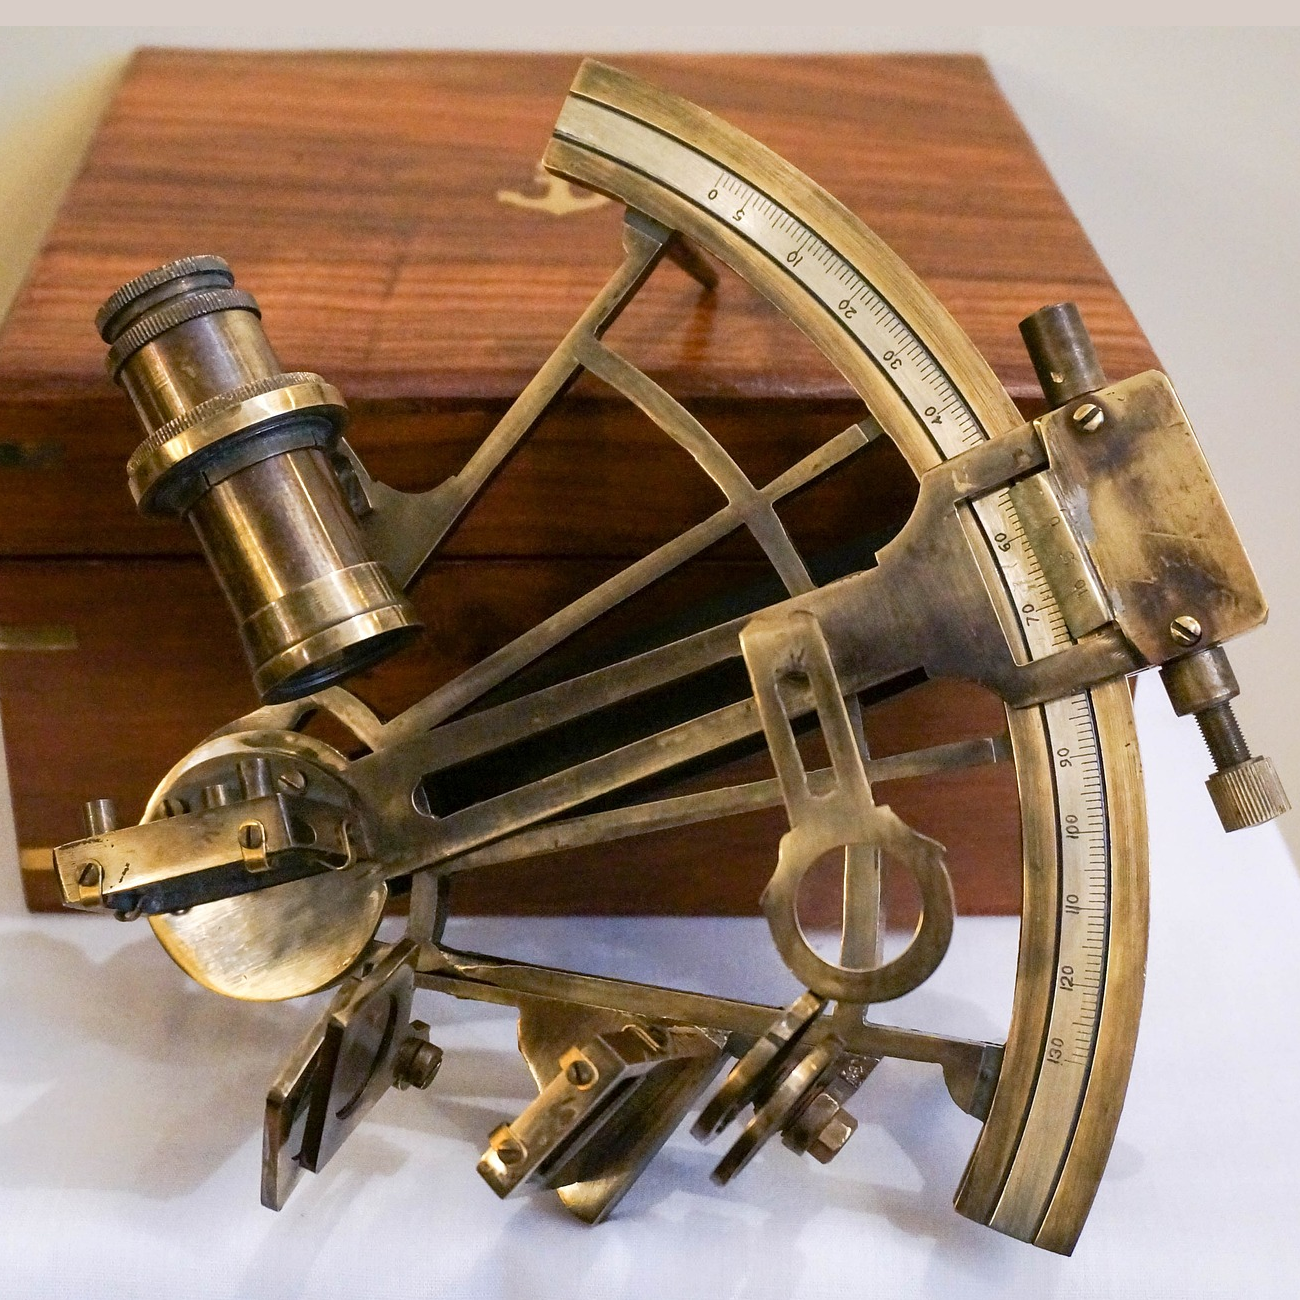
\includegraphics[width=\textwidth]{../SurvivalItemImages/sextant}
        \end{minipage}\hfill
        \begin{minipage}{0.7\textwidth}
            \centering
            \Large A sextant
        \end{minipage}
    \end{figure}
    \vspace{-0.8em}
    \noindent\rule{\textwidth}{0.4pt}
            
    \begin{figure}[H]
        \centering
        \begin{minipage}{0.25\textwidth}
            \centering
            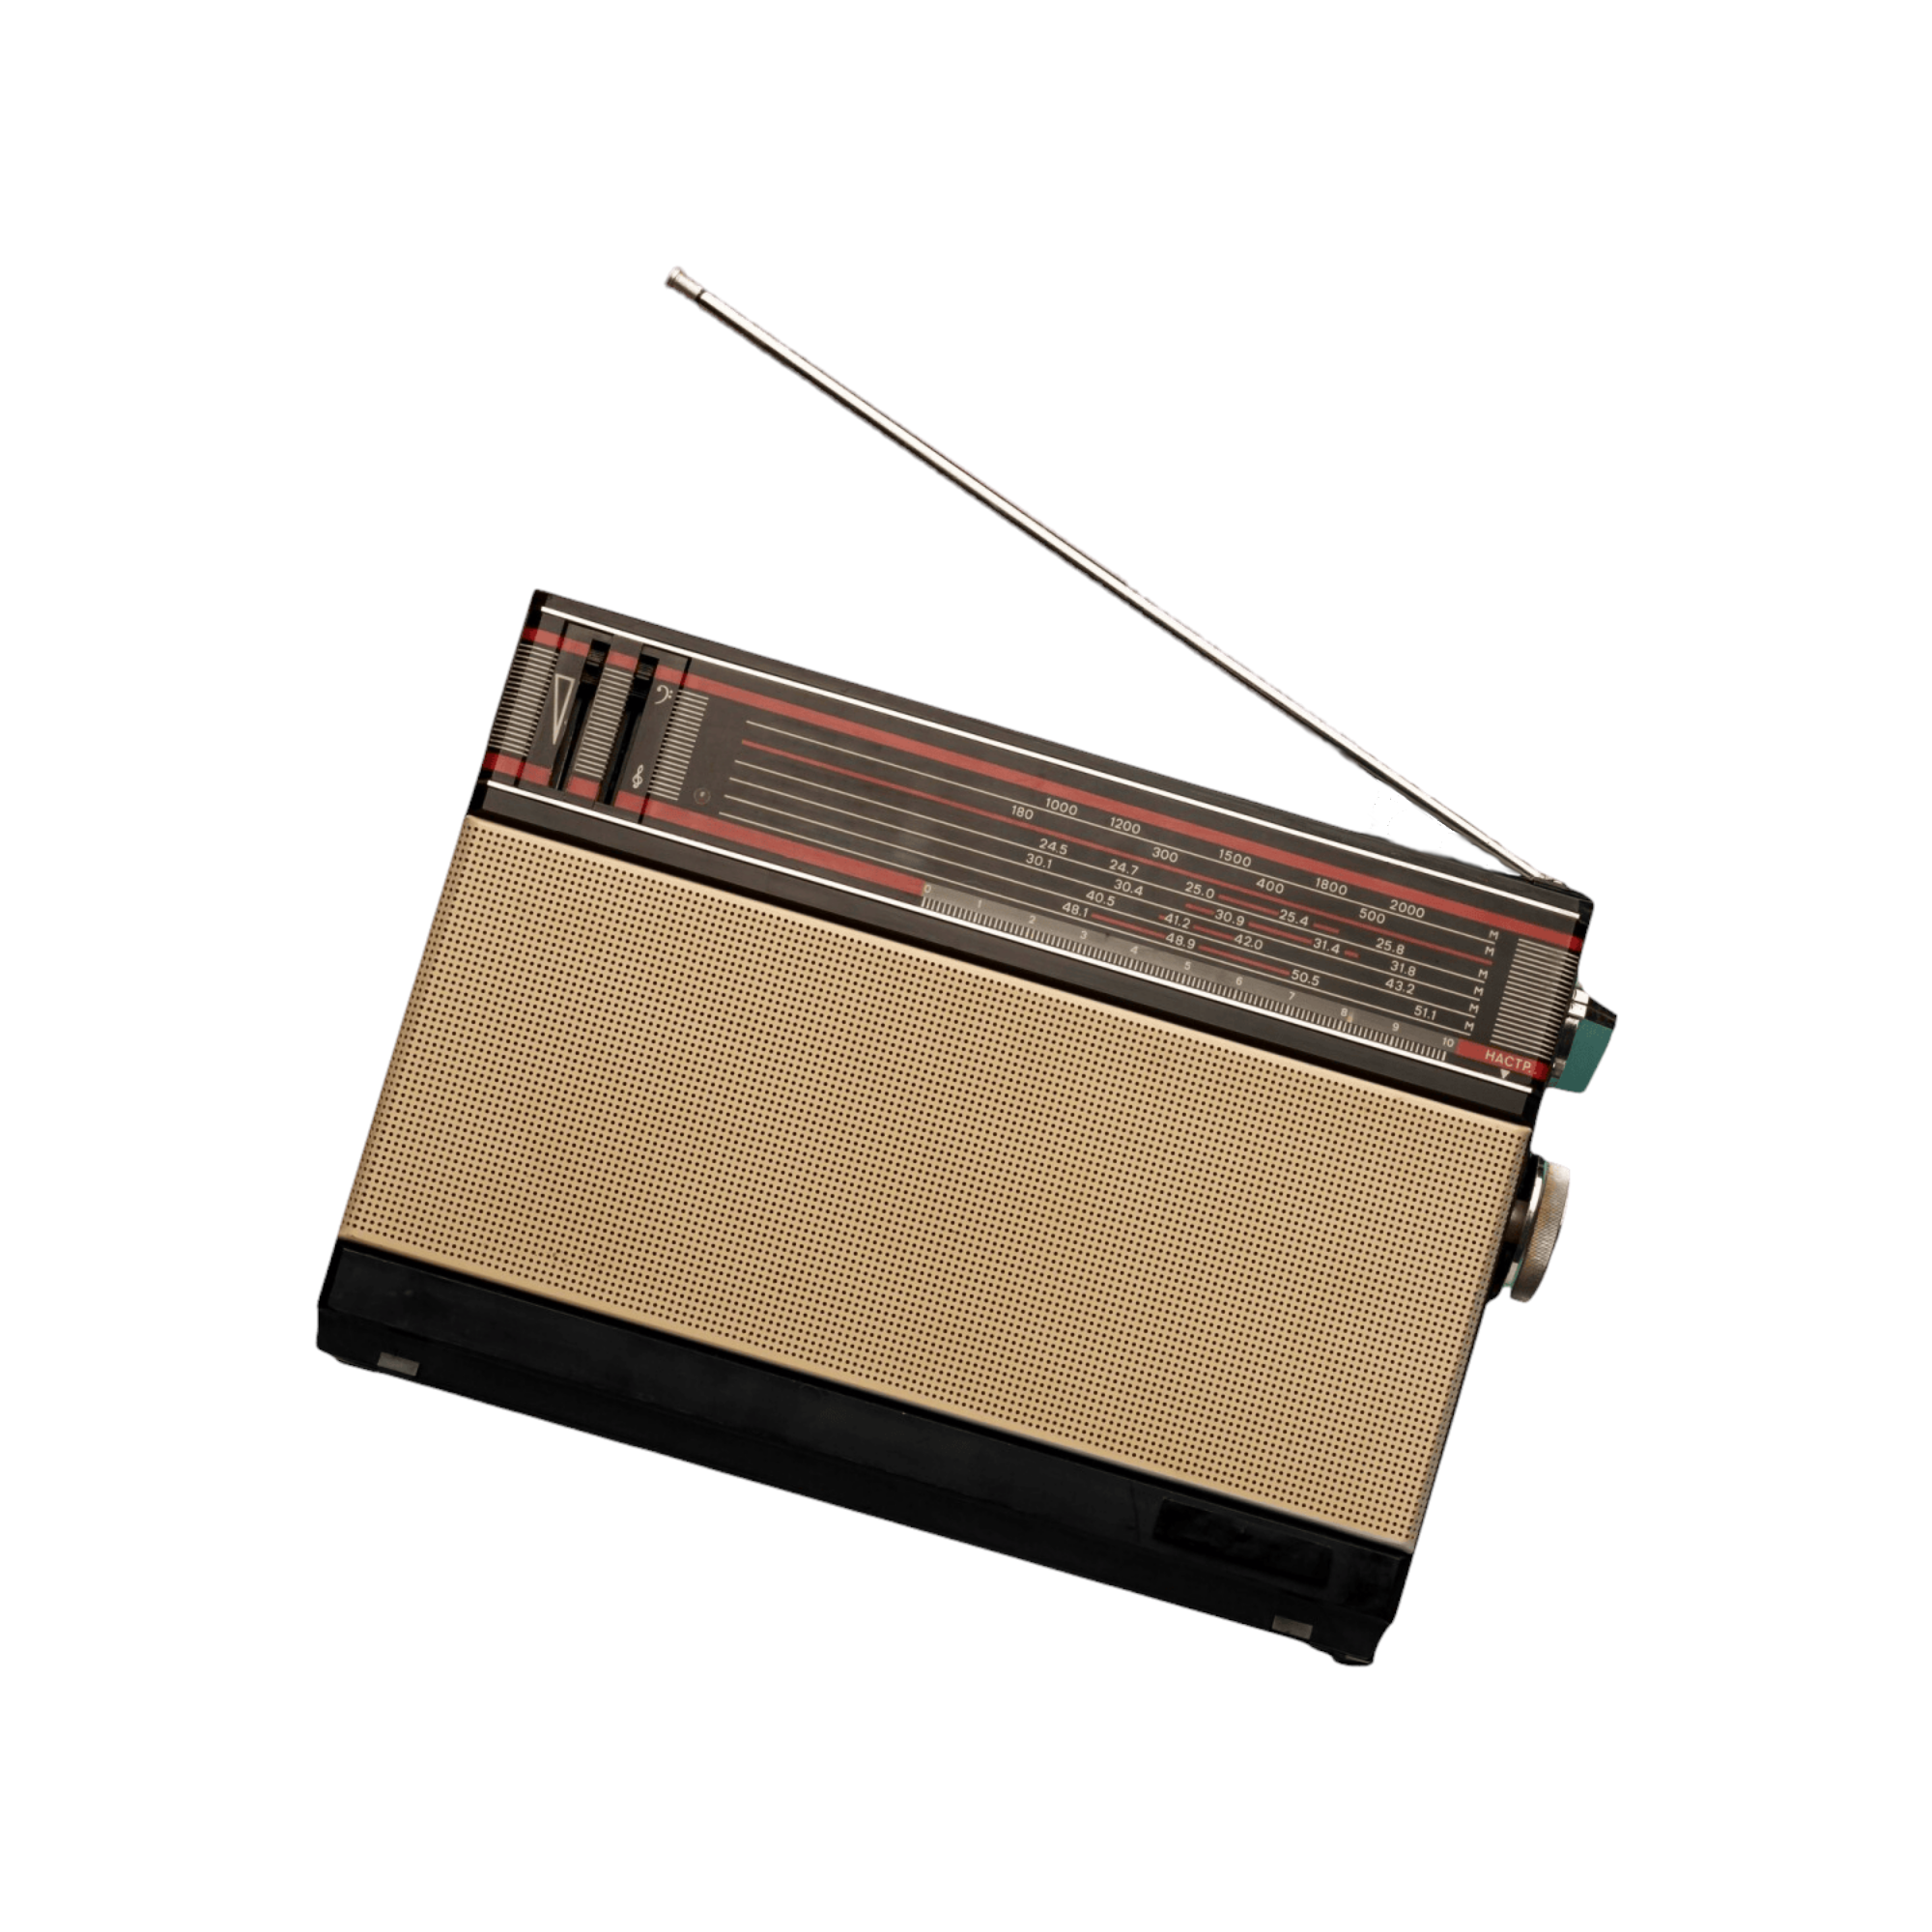
\includegraphics[width=\textwidth]{../SurvivalItemImages/radio}
        \end{minipage}\hfill
        \begin{minipage}{0.7\textwidth}
            \centering
            \Large A small transistor radio
        \end{minipage}
    \end{figure}
    \vspace{-0.8em}
    \noindent\rule{\textwidth}{0.4pt}
            
    \begin{figure}[H]
        \centering
        \begin{minipage}{0.25\textwidth}
            \centering
            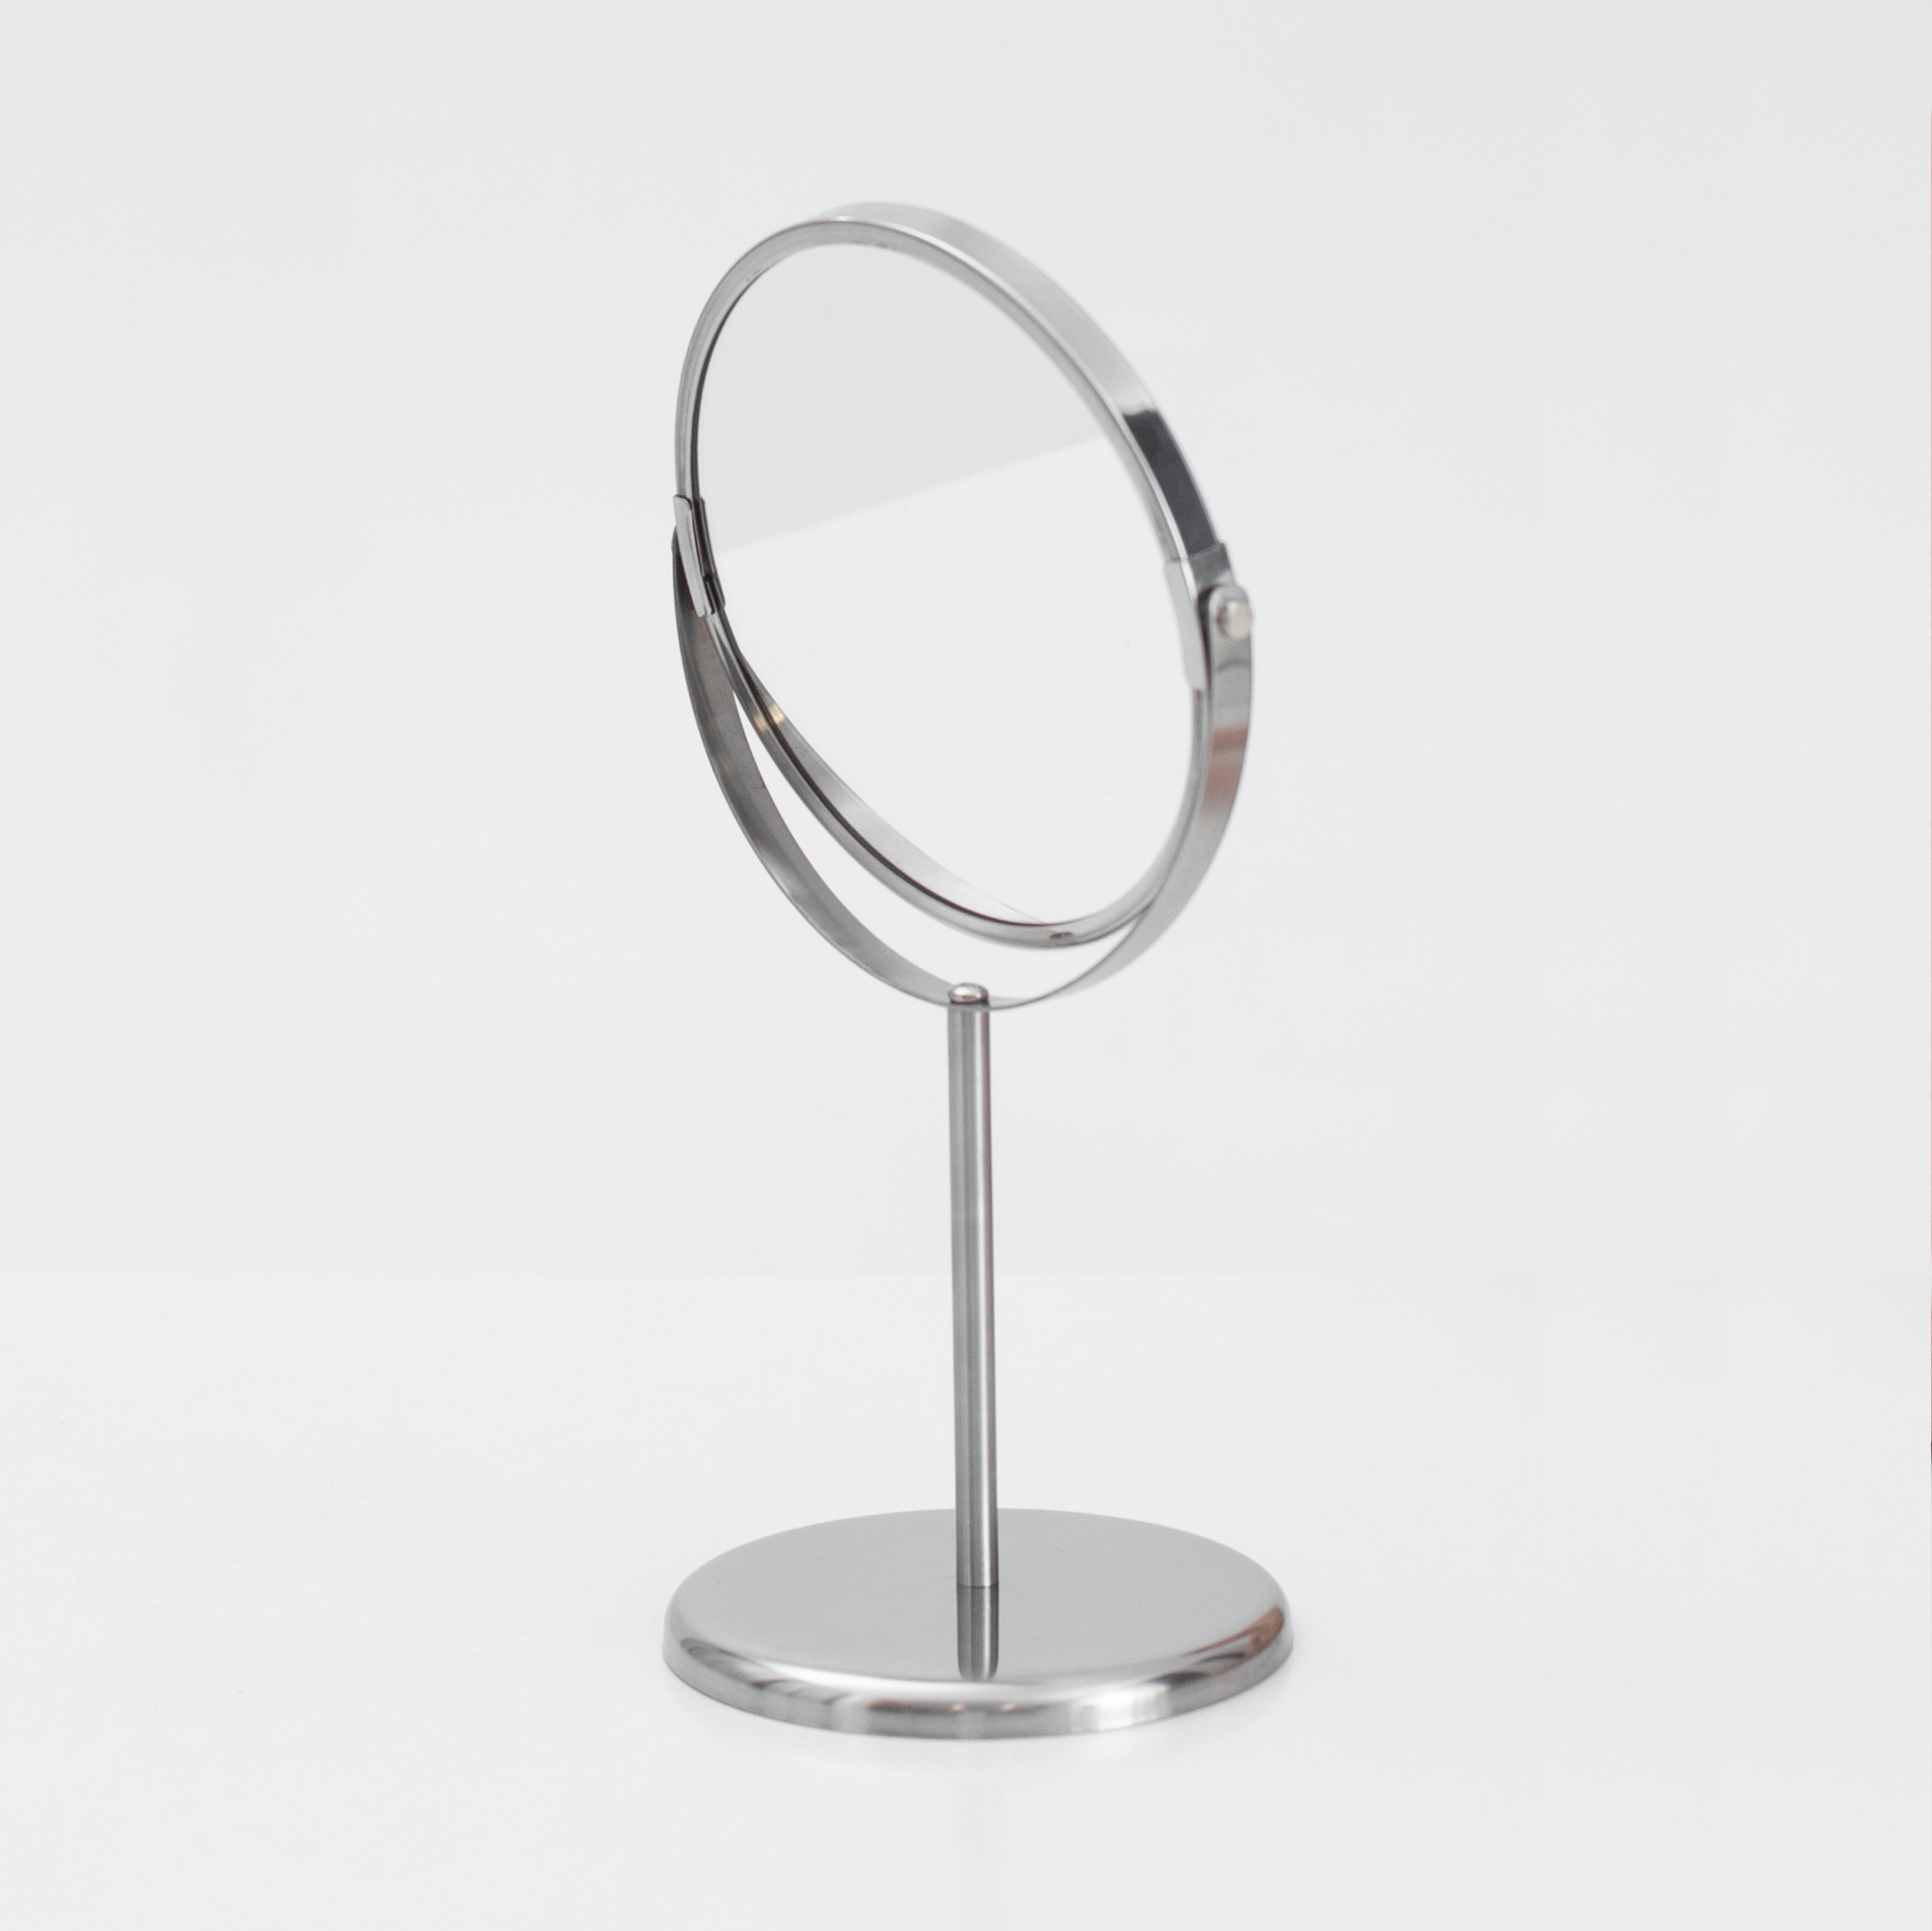
\includegraphics[width=\textwidth]{../SurvivalItemImages/mirror}
        \end{minipage}\hfill
        \begin{minipage}{0.7\textwidth}
            \centering
            \Large A shaving mirror
        \end{minipage}
    \end{figure}
    \vspace{-0.8em}
    \noindent\rule{\textwidth}{0.4pt}
            
    \begin{figure}[H]
        \centering
        \begin{minipage}{0.25\textwidth}
            \centering
            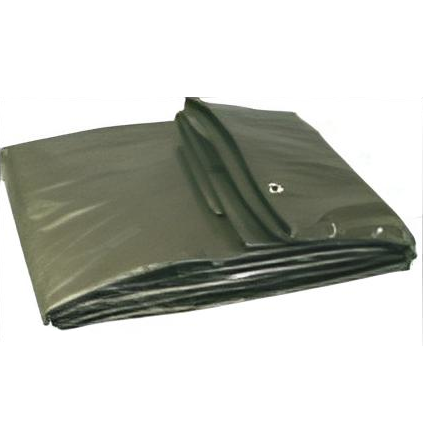
\includegraphics[width=\textwidth]{../SurvivalItemImages/plasticsheeting}
        \end{minipage}\hfill
        \begin{minipage}{0.7\textwidth}
            \centering
            \Large 20 square feet of Opaque plastic sheeting
        \end{minipage}
    \end{figure}
    \vspace{-0.8em}
    \noindent\rule{\textwidth}{0.4pt}
            
    \clearpage
    \section*{Scenario: \textmd{Sea} \hfill Participant \textmd{0}}
    \Large You are drifting in a private yacht in the South Pacific. A fire with unknown origin has destroyed much of the yacht, notably navigational and radio equipment. After having controlled the fire, you realize that the boat is sinking little by little. Your best estimate is that you are many hundreds of miles from the nearest landfall. You and your friends have managed to save 15 items, undamaged and intact after the fire. In addition, you have salvaged a four man rubber life craft and a box of matches.
\clearpage
        \par\noindent\rule{\textwidth}{0.4pt}
    \begin{figure}[H]
        \centering
        \begin{minipage}{0.25\textwidth}
            \centering
            \includegraphics[width=\textwidth]{../SurvivalItemImages/water20l}
        \end{minipage}\hfill
        \begin{minipage}{0.7\textwidth}
            \centering
            \Large A 20 litre container of water 
        \end{minipage}
    \end{figure}
    \vspace{-0.8em}
    \noindent\rule{\textwidth}{0.4pt}
            
    \begin{figure}[H]
        \centering
        \begin{minipage}{0.25\textwidth}
            \centering
            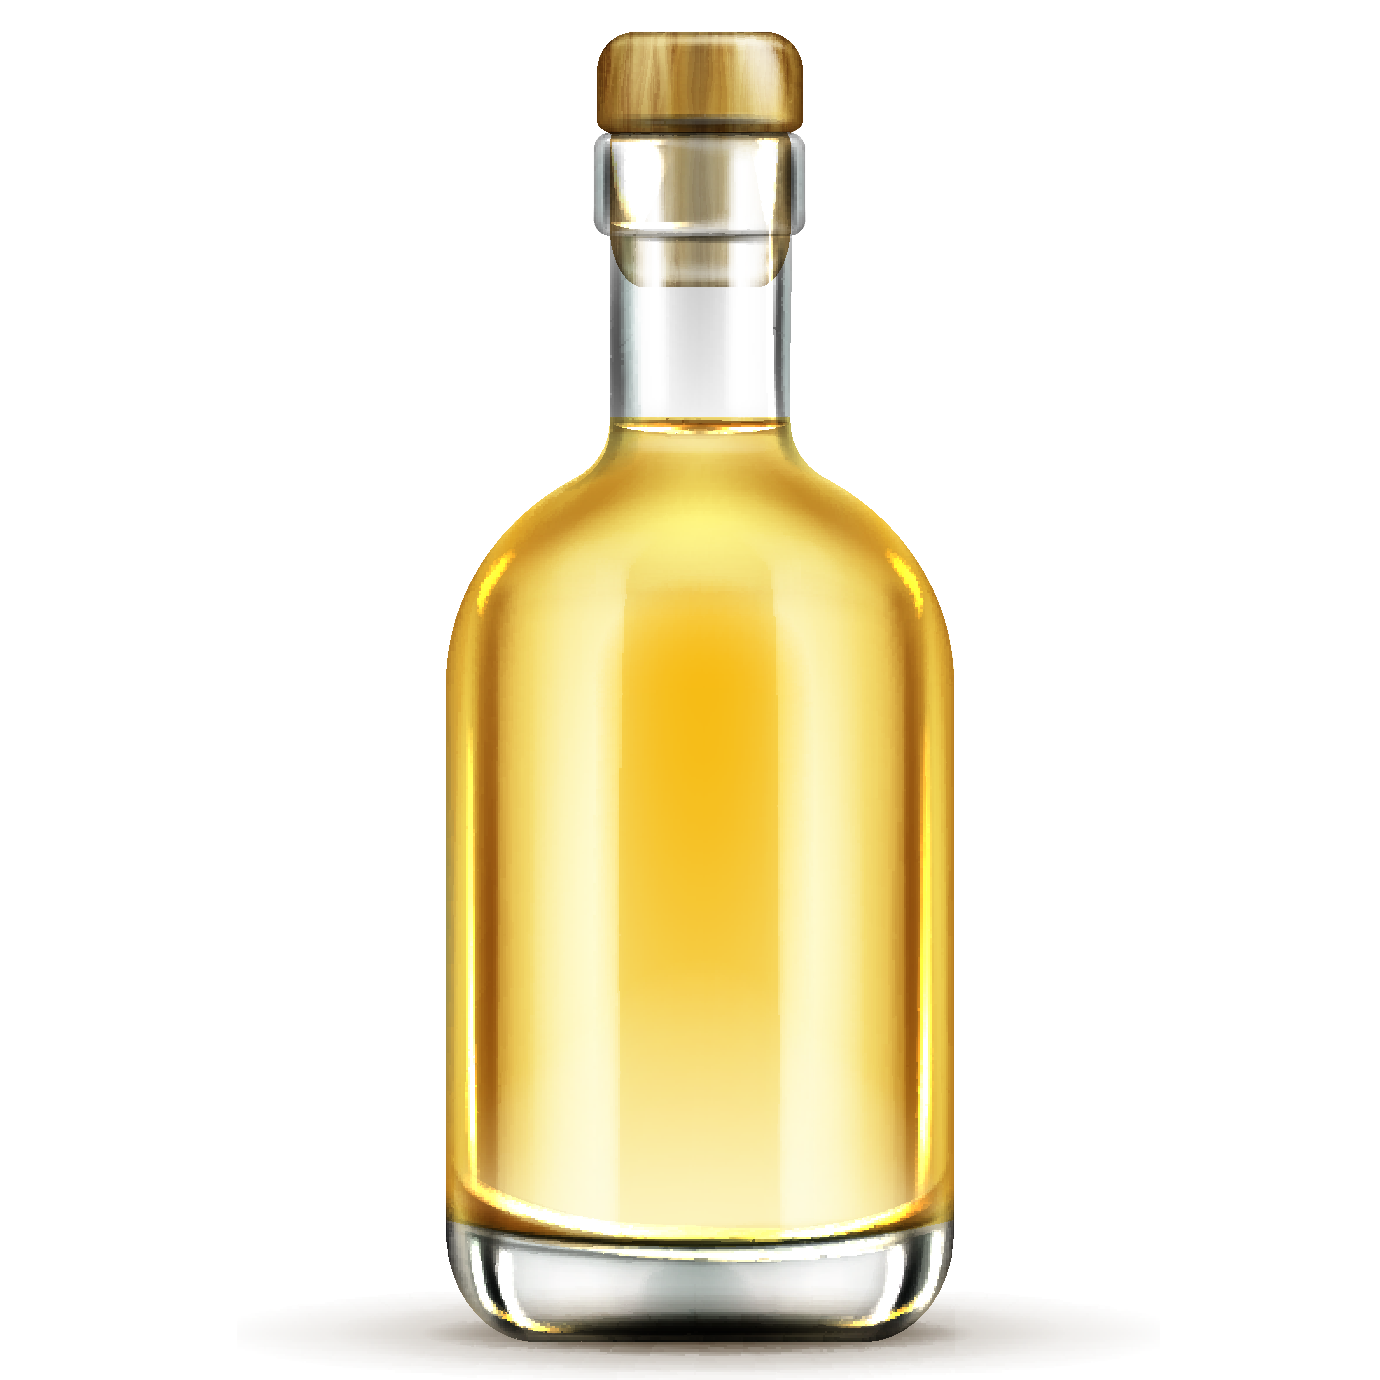
\includegraphics[width=\textwidth]{../SurvivalItemImages/strongrum}
        \end{minipage}\hfill
        \begin{minipage}{0.7\textwidth}
            \centering
            \Large One bottle of 160 per cent proof rum
        \end{minipage}
    \end{figure}
    \vspace{-0.8em}
    \noindent\rule{\textwidth}{0.4pt}
            
    \begin{figure}[H]
        \centering
        \begin{minipage}{0.25\textwidth}
            \centering
            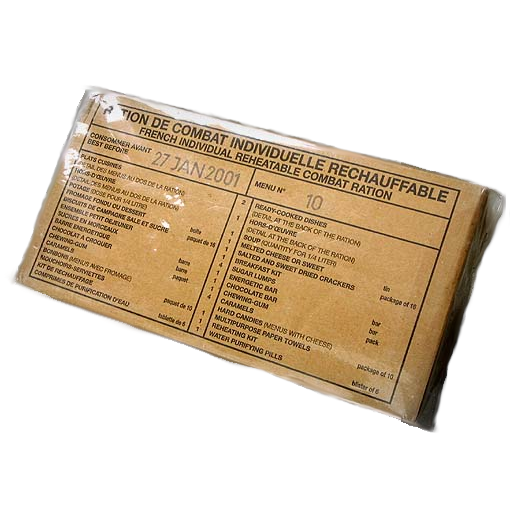
\includegraphics[width=\textwidth]{../SurvivalItemImages/rations}
        \end{minipage}\hfill
        \begin{minipage}{0.7\textwidth}
            \centering
            \Large A case of army rations
        \end{minipage}
    \end{figure}
    \vspace{-0.8em}
    \noindent\rule{\textwidth}{0.4pt}
            
    \begin{figure}[H]
        \centering
        \begin{minipage}{0.25\textwidth}
            \centering
            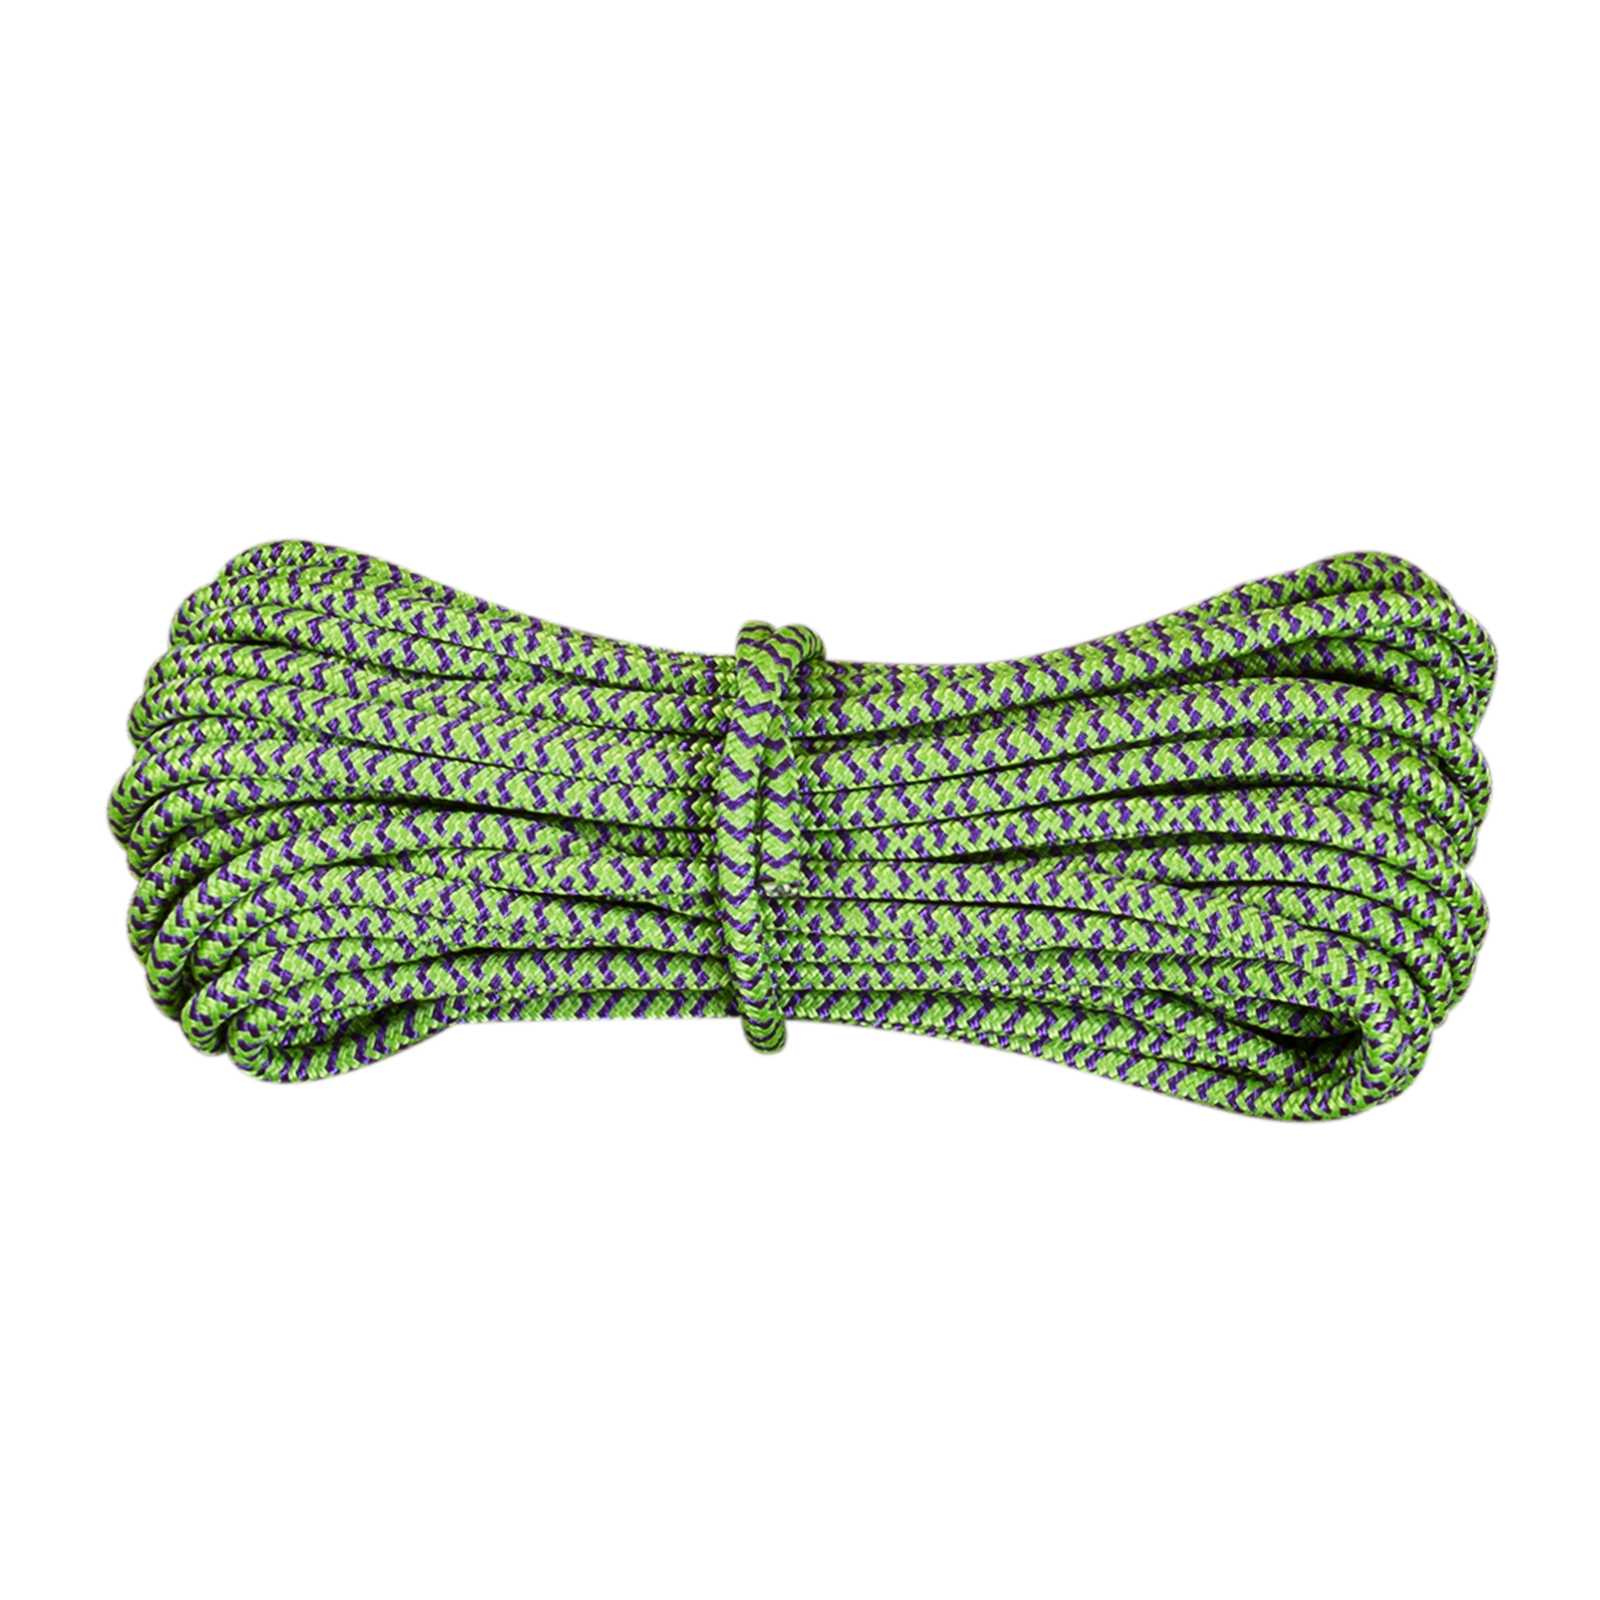
\includegraphics[width=\textwidth]{../SurvivalItemImages/rope}
        \end{minipage}\hfill
        \begin{minipage}{0.7\textwidth}
            \centering
            \Large 15ft nylon rope
        \end{minipage}
    \end{figure}
    \vspace{-0.8em}
    \noindent\rule{\textwidth}{0.4pt}
            
    \clearpage
    \section*{Scenario: \textmd{Sea} \hfill Participant \textmd{1}}
    \Large You are drifting in a private yacht in the South Pacific. A fire with unknown origin has destroyed much of the yacht, notably navigational and radio equipment. After having controlled the fire, you realize that the boat is sinking little by little. Your best estimate is that you are many hundreds of miles from the nearest landfall. You and your friends have managed to save 15 items, undamaged and intact after the fire. In addition, you have salvaged a four man rubber life craft and a box of matches.
\clearpage
        \par\noindent\rule{\textwidth}{0.4pt}
    \begin{figure}[H]
        \centering
        \begin{minipage}{0.25\textwidth}
            \centering
            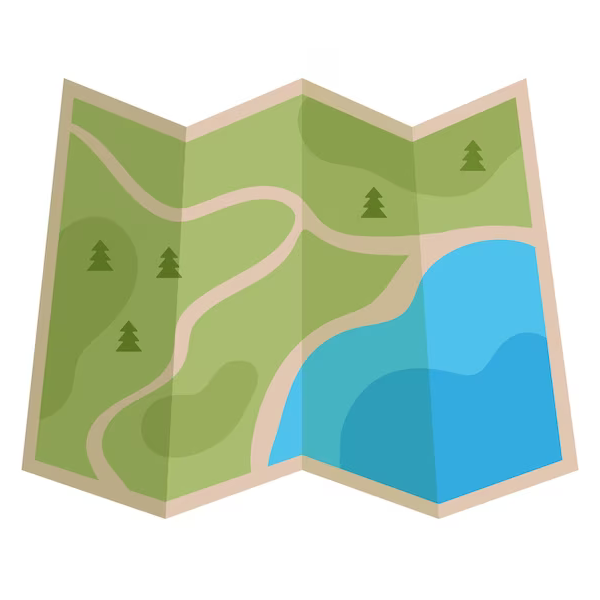
\includegraphics[width=\textwidth]{../SurvivalItemImages/seamap}
        \end{minipage}\hfill
        \begin{minipage}{0.7\textwidth}
            \centering
            \Large A map of the Pacific Ocean
        \end{minipage}
    \end{figure}
    \vspace{-0.8em}
    \noindent\rule{\textwidth}{0.4pt}
            
    \begin{figure}[H]
        \centering
        \begin{minipage}{0.25\textwidth}
            \centering
            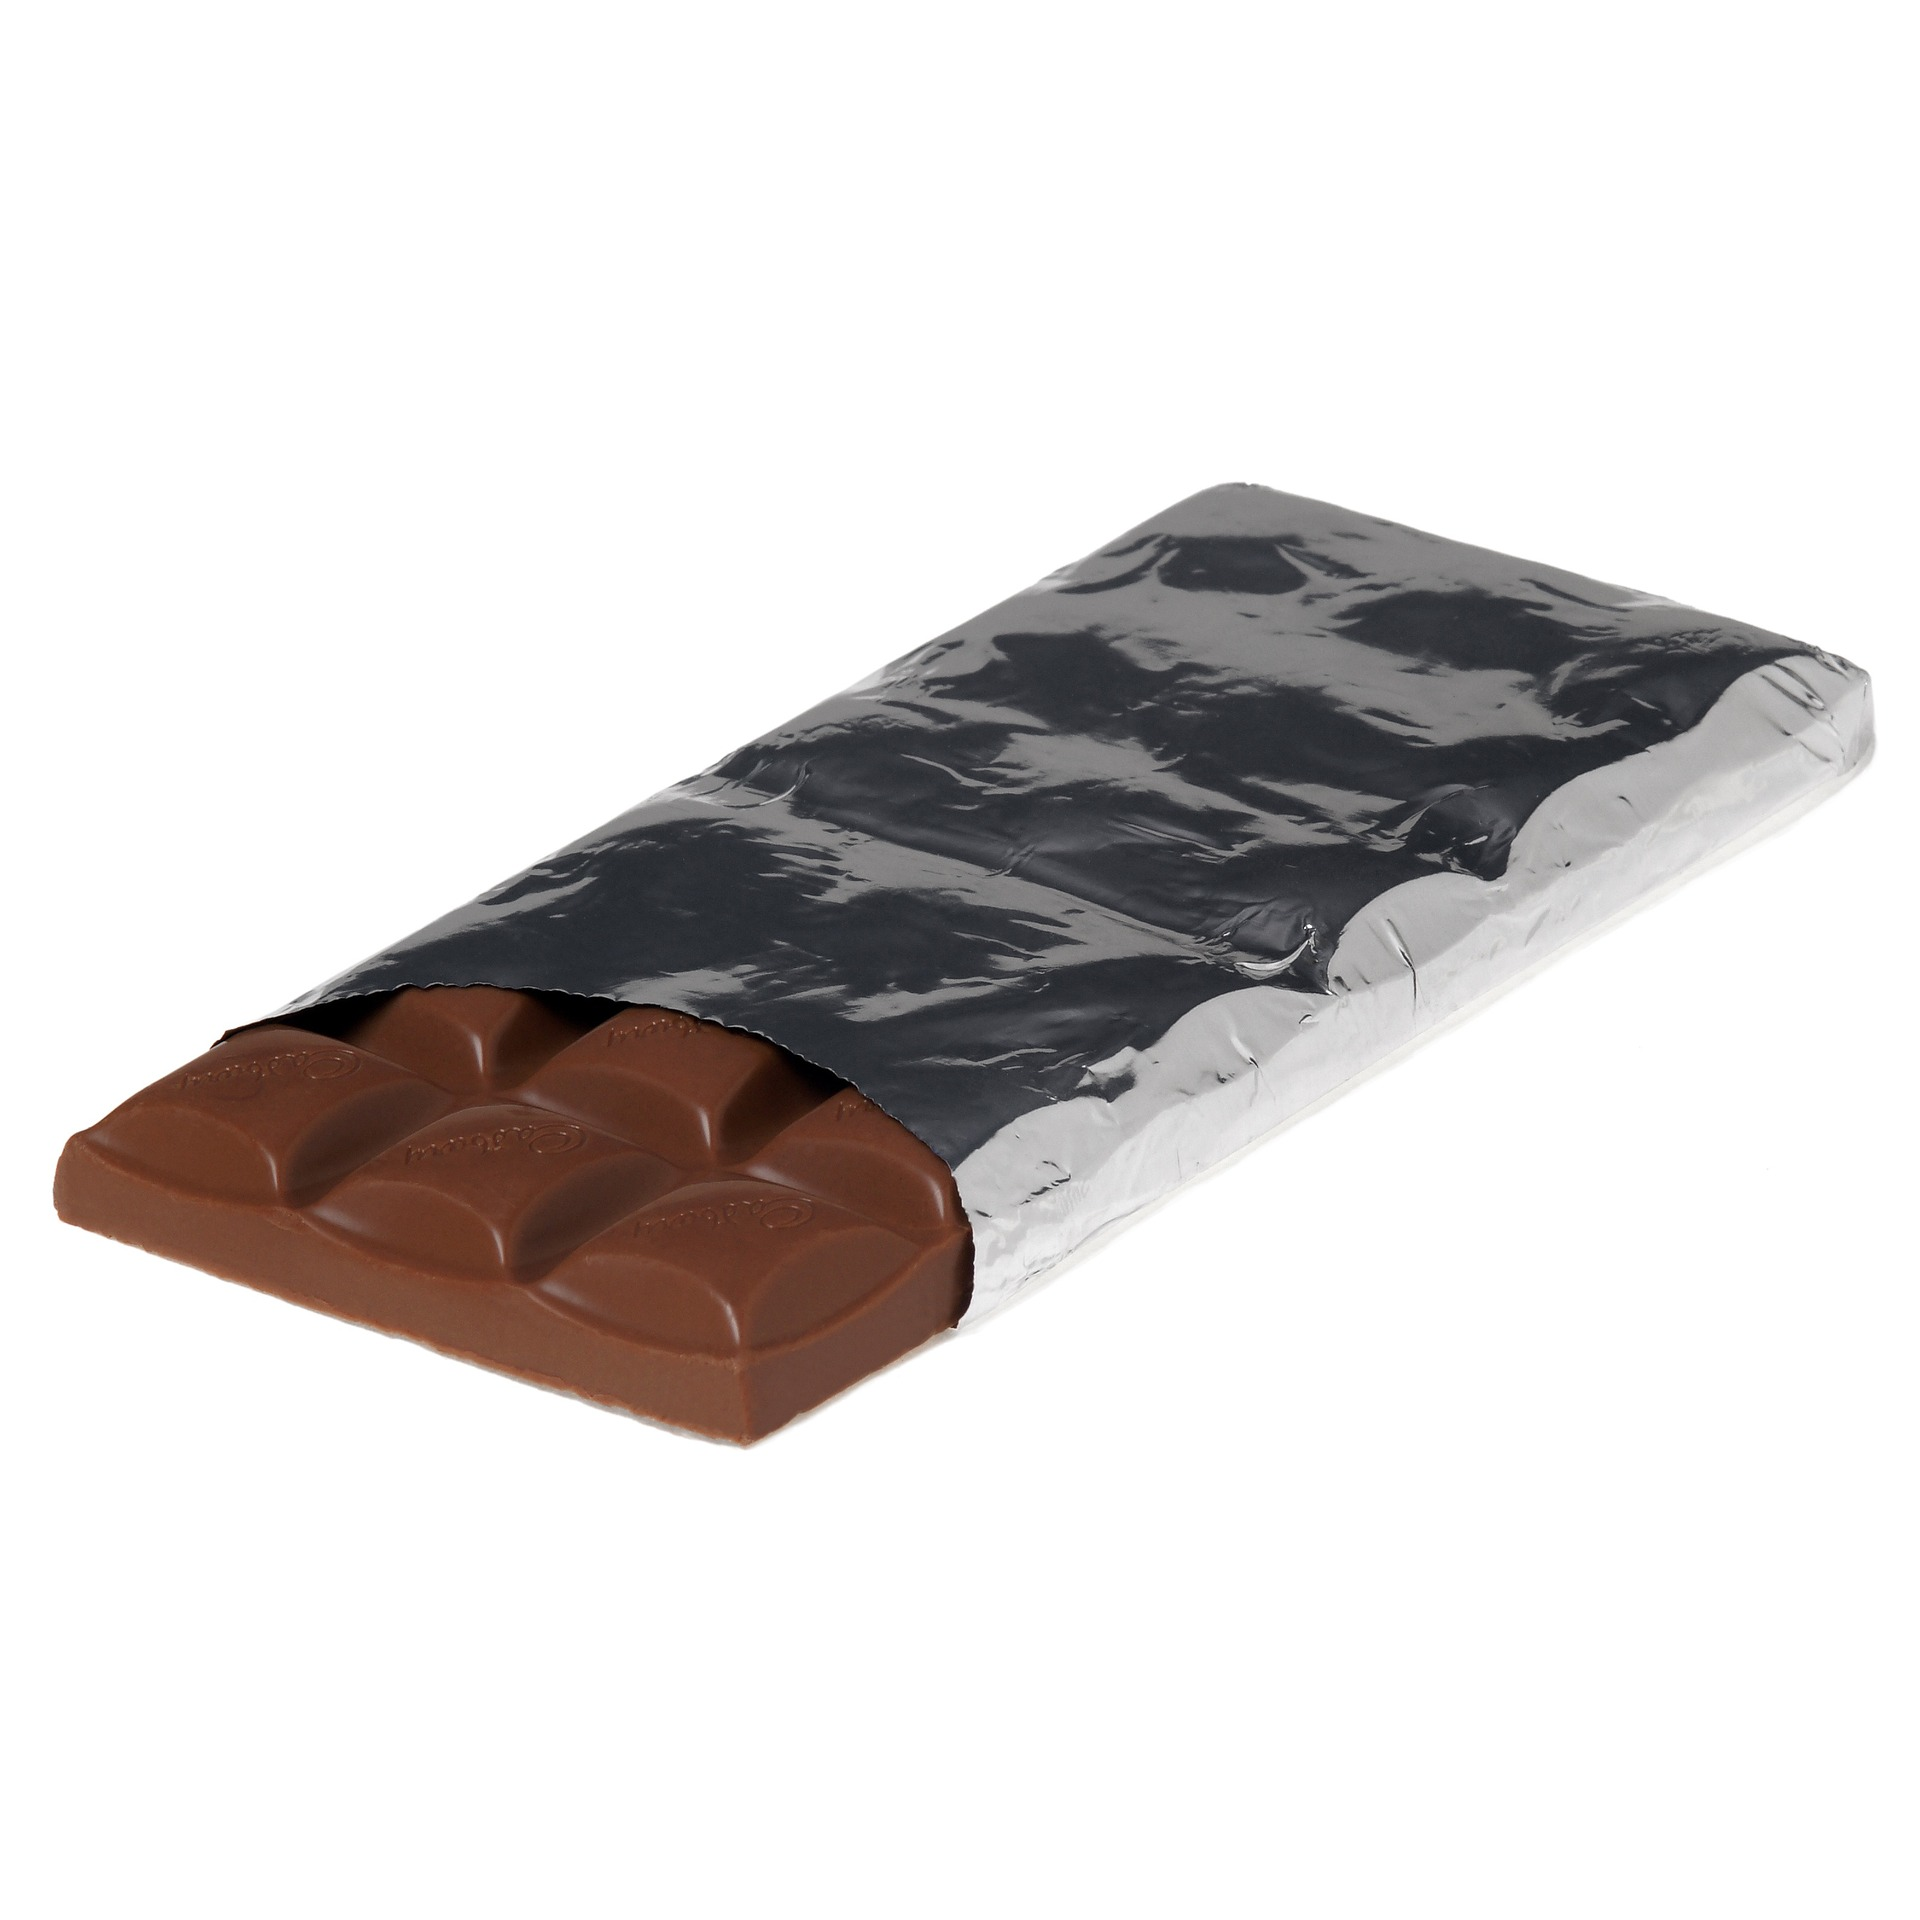
\includegraphics[width=\textwidth]{../SurvivalItemImages/chocolate}
        \end{minipage}\hfill
        \begin{minipage}{0.7\textwidth}
            \centering
            \Large 2 boxes of chocolate bars
        \end{minipage}
    \end{figure}
    \vspace{-0.8em}
    \noindent\rule{\textwidth}{0.4pt}
            
    \begin{figure}[H]
        \centering
        \begin{minipage}{0.25\textwidth}
            \centering
            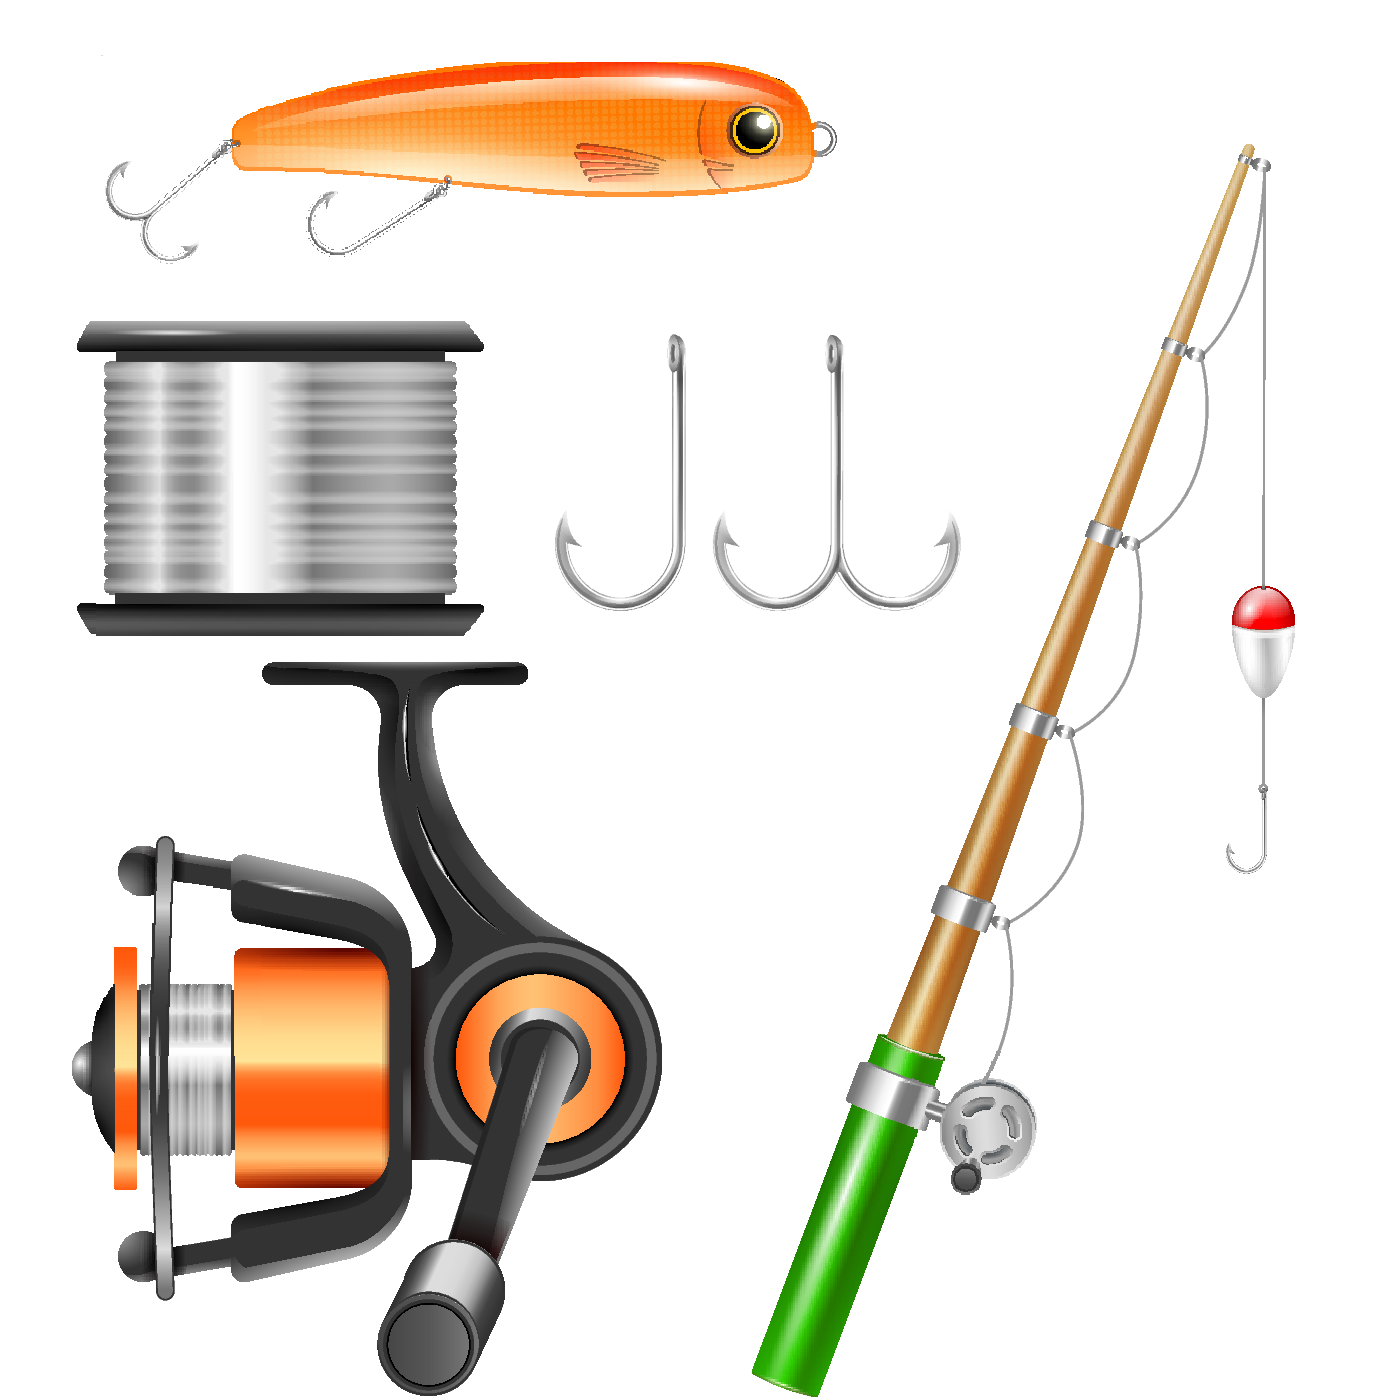
\includegraphics[width=\textwidth]{../SurvivalItemImages/fishingkit}
        \end{minipage}\hfill
        \begin{minipage}{0.7\textwidth}
            \centering
            \Large A fishing kit
        \end{minipage}
    \end{figure}
    \vspace{-0.8em}
    \noindent\rule{\textwidth}{0.4pt}
            
    \begin{figure}[H]
        \centering
        \begin{minipage}{0.25\textwidth}
            \centering
            \includegraphics[width=\textwidth]{../SurvivalItemImages/oilcanister}
        \end{minipage}\hfill
        \begin{minipage}{0.7\textwidth}
            \centering
            \Large A 7 litre can of oil/petrol mixture
        \end{minipage}
    \end{figure}
    \vspace{-0.8em}
    \noindent\rule{\textwidth}{0.4pt}
            
    \clearpage
    \section*{Scenario: \textmd{Sea} \hfill Participant \textmd{2}}
    \Large You are drifting in a private yacht in the South Pacific. A fire with unknown origin has destroyed much of the yacht, notably navigational and radio equipment. After having controlled the fire, you realize that the boat is sinking little by little. Your best estimate is that you are many hundreds of miles from the nearest landfall. You and your friends have managed to save 15 items, undamaged and intact after the fire. In addition, you have salvaged a four man rubber life craft and a box of matches.
\clearpage
        \end{document}
        